\begin{tikzpicture}[>=stealth, font=\small,
    neuron/.style={circle, draw=black!60, inner sep=0pt, minimum size=6pt},
    box/.style={rounded corners=4pt, draw=blue!50!black, thick, align=center}]
    % network with two sigmoid heads
    \foreach \y [count=\i] in {0.6, 0.2, -0.2, -0.6} \node[neuron, fill=yellow!60] (i\i) at (0.5, \y) {};
    \foreach \y [count=\i] in {0.9, 0.45, 0, -0.45, -0.9} \node[neuron, fill=cyan!45] (h\i) at (1.2, \y) {};
    \foreach \y [count=\i] in {0.9, 0.45, 0, -0.45, -0.9} \node[neuron, fill=cyan!45] (k\i) at (1.9, \y) {};
    \foreach \y [count=\i] in {1.3, 0.95, 0.6} \node[neuron, fill=red!40] (o\i) at (2.6, \y) {};
    \foreach \y [count=\i] in {-0.6, -0.95, -1.3} \node[neuron, fill=orange!55] (a\i) at (2.6, \y) {};
    \foreach \a in {1,...,4} \foreach \b in {1,...,5} \draw[black!20] (i\a) -- (h\b);
    \foreach \a in {1,...,5} \foreach \b in {1,...,5} \draw[black!20] (h\a) -- (k\b);
    \foreach \a in {1,...,5} \foreach \b in {1,2,3} {\draw[black!20] (k\a) -- (o\b); \draw[black!20] (k\a) -- (a\b);}
    \draw[->, thick] (-0.3,0) node[left] {$(\boldsymbol{d}, R)$} -- (0.3,0);
    \node[font=\footnotesize] at (1.5,-1.6) {DNN, two sigmoid heads};
    % repair layers of E2ELR on each head
    \node[box, fill=green!15, text width=3.0cm, minimum height=0.85cm, font=\footnotesize] (rd) at (6.0,0.95) {Power balance and\\ reserve layers};
    \node[box, fill=green!15, text width=3.0cm, minimum height=0.85cm, font=\footnotesize] (ra) at (6.0,-0.95) {Power balance and\\ reserve layers};
    \draw[->, thick] (2.8,0.95) -- node[above, font=\footnotesize] {dispatch} (rd.west);
    \draw[->, thick] (2.8,-0.95) -- node[below, font=\footnotesize] {anchor} (ra.west);
    % line flow repair layer
    \node[box, fill=violet!12, text width=4.5cm, minimum height=2.7cm] (lr) at (10.7,0) {\textbf{Line flow repair layer}\\[6pt]
        $\hat{\boldsymbol{p}} = (1 - \alpha) \tilde{\boldsymbol{p}} + \alpha \boldsymbol{p}^a$\\[4pt]
        $\alpha = \max\limits_{(i,j) \in \mathcal{E}} \dfrac{o_{ij}}{o_{ij} + s_{ij}}$};
    \draw[->, thick] (rd.east) -- node[above] {$\tilde{\boldsymbol{p}}$} (lr.west |- rd.east);
    \draw[->, thick] (ra.east) -- node[below] {$\boldsymbol{p}^a$} (lr.west |- ra.east);
    \draw[->, thick] (lr.east) -- node[above] {$\hat{\boldsymbol{p}}, f^a$} (13.9,0) node[right] {$\mathcal{L}(\hat{\boldsymbol{p}}, f^a)$};
    % backpropagation
    \draw[->, dashed, thick, orange!80!black] (14.9,-0.3) -- (14.9,-2.05) -- (1.5,-2.05) -- (1.5,-1.8);
    \node[orange!80!black, below, font=\footnotesize\bfseries] at (8.2,-2.05) {Backpropagation};
\end{tikzpicture}
